\section{設計} \label{section:design}


\sysname は,上記の設計上の課題に対するソフトウェアレベルの解決策を提供する.
コンポーネント単位で効率的に Unikernel を若返らせるために,
\sysname は各コンポーネントごとの専用のスレッドを用意し,
コンポーネントの若返りが
他のコンポーネントの実行に影響を与えるのを防ぐ.

関係のあるコンポーネントの動作状態に影響を与えるのを防ぐため,
\sysname は,ログの再生時に,再起動したコンポーネントをカプセル化する.
また,\sysname は,コンポーネント初期化後に取得したコンポーネントのメモリスナップショットを使用し,
選択的に対象のコンポーネントの状態を変化させる関数のみを実行します.


\subsection{マルチスレッド Unikernel コンポーネント}

Unikernel をコンポーネント単位で若返えらせるために,
Unikernel コンポーネントの実行について考慮する必要がある.
Unikernel は,ライブラリのように動作するため,
各コンポーネントはその機能を呼び出すスレッドコンテキストによって実行される.
Unikernel にリンクされたアプリケーションのスレッドがファイルを開くことを要求すると,
そのコンテキストは,ファイルシステム関連のコンポーネントを実行する.
本来のアプローチでは,スレッドコンテキストが対象のコンポーネントに到達したときに
そのコンポーネントを若返らせる.
この方法は,その実行に直接影響を与えるため,現在のコンテキストに関係ないコンポーネントを若返らせることができなくなる,
例えば,Unikernel にリンクされたアプリケーションがファイル関連の処理を実行している間は,
ネットワークコンポーネントを若返らせることができない.

この問題を解決するために,
\sysname はすべてのコンポーネントに専用のスレッドを割り当てて,
メッセージパッシング方式で相互に交流する.
この方式は,アプリケーションのコンテキストに対して, \sysname のコンポーネントの透過的な若返りを可能にする.
例えば,\sysname は,アプリケーションスレッドが使用していないコンポーネントを若返らせることができ,
若返りがアプリケーションの行動に影響を与えるのを防ぐ.
そして,再起動されたコンポーネントの動作状態を復元することで,
\sysname にリンクされたアプリケーションが再起動に渡って動作を継続し続けることができる.

\sysname のコンポーネントは,
それぞれ自身のデータ領域とヒープ領域を保持し,
自身に実装されている関数は,
呼び出し元コンポーネントのスレッドではなく,
自身に割り当てられている専用のスレッドによって実行される.
各スレッドは,
他のコンポーネントの関数の引数を呼び出し先のコンポーネントに渡すことにより,
その関数を呼び出し,関数の実行には,コンポーネントごとのデータ領域とヒープ領域が使われる.
通常の Unikernel では,アプリケーションがファイルを開くために,VFS (仮想ファイルシステム)のコンポーネントが公開する \textbf{open()} を呼び出す際には,
アプリケーションのスレッドコンテキストが VFS コンポーネントの \textbf{open()} へとジャンプする.
一方で, VampOS にリンクされたアプリケーションがファイルを開くには,
アプリケーションのスレッドが \textbf{open()} の引数を VFS コンポーネントに渡し,
VFS コンポーネントのスレッドが \textbf{open()} を実行する.
\sysname が引数を取り出するために,コンポーネントによって公開されたインタフェースをフックし,
呼び出し先のコンポーネントのメモリにその引数をコピーする.
関数の実行中に参照される引数は,
呼び出し元のコンポーネントのメモリにあるものではなく,
自身のメモリ上の複製されたものである.


\subsection{コンポーネントの若返り}

Unikernel のコンポーネント単位の若返りにおいて,
対象のコンポーネントの動作状態に注意を払う.
ファイルシステムやネットワークのような多くの OS サブシステムが状態を持ち,
それらの状態持つ Unikernel コンポーネントの再起動が
アプリケーションと他のコンポーネントが継続して動作させることができない.
例えば,ファイルオフセットを保持する VFS コンポーネントを若返りさせると,
ファイルオフセットが 0 に初期化されるため,
若返り後のアプリケーションのファイル操作を正しく行えなくなる.
ソフトウェア若化の観点から,
対象のコンポーネントのメモリスナップショットを再起動の直前に取得し,
動作状態を復元するのは意味がない.
なぜなら,
メモリリークやディスクリプタリーク,メモリフラグメンテーションを含む
古くなったメモリイメージが再作成されるからである.

\begin{figure}[t]
    \centering
    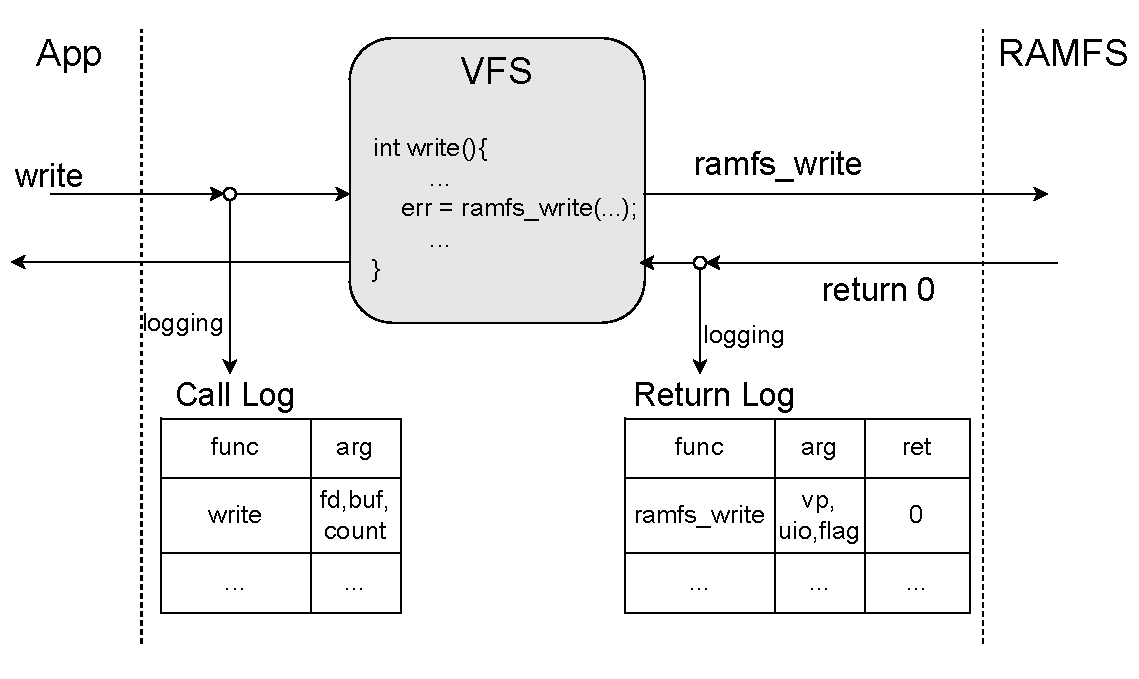
\includegraphics[width=\linewidth]{img/logging.pdf}
    \vspace{-5mm}
    \caption{\textbf{コンポーネント間のインタフェースのロギング.} \textit{他のコンポーネントに対して透過的に若返りしたコンポーネントの動作状態を復元するために,{\sysname} はコンポーネントが公開するインタフェースをフックし,関数呼び出しを記録した後,値を返す..}}
    \label{fig:logging}
\end{figure}

\begin{figure}[t]
    \centering
    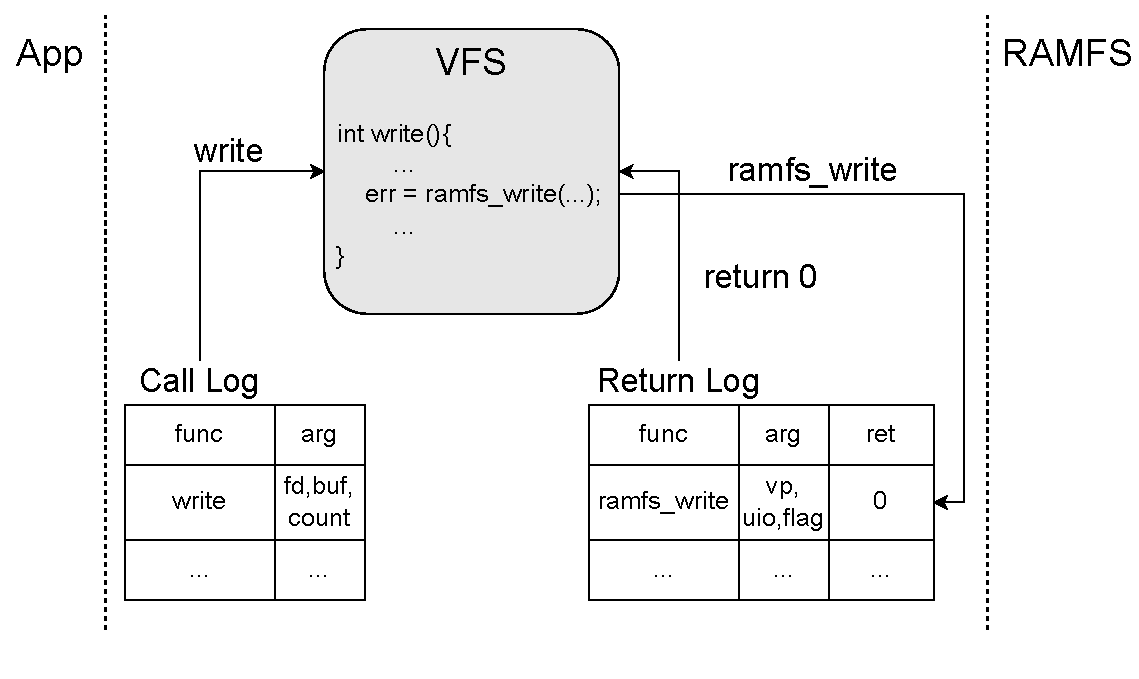
\includegraphics[width=\linewidth]{img/playlog.pdf}
    \caption{\textbf{コンポーネントの復元のためのログの再生.} \textit{コンポーネントの再起動の後に,\sysname は状態を変化させる関数を実行させる.その際,他のコンポーネントの関数呼び出しの戻り値を再利用することで,その実行による他のコンポーネントの動作状態の変化を防ぐ.}}
    \label{fig:restoration}
\end{figure}

状態を持つコンポーネントの若返りによって生じる不整合を防ぎため,
再起動の後に状態を持つコンポーネントの動作状態を復元する.
復元のために,\sysname は,他のコンポーネントからの対象の関数に対する関数呼び出しを記録し,
若返りの後にコンポーネントのログを再生する.
図\ref{fig:logging}は,\sysname のコンポーネント間のインタラクションのロギングを示している.
若返り前に実行されたすべての関数を再実行するのではなく,
復元の時間の短縮およびメモリリークやメモリフラグメンテーションのような老化関連のバグによるエラー状態の再現を防ぐため,
\sysname は選択的に関数を呼び出す.
\sysname は,若返りの直前の状態を復元するのに必要な関数のみを呼び出す.
具体的には,ファイル状態の読み出し(\textbf{fstat()} 関連の関数)のようなコンポーネントの状態を変更しない関数は,
呼び出されない.
また,\sysname はすでに閉じられたファイルへの操作といった
コンポーネントの現在の状態を生成しない関数を再実行しない・

\subsection{チェックポイントベースの若返り}

シャットダウンやブート処理を行う
通常のコンポーネントの再起動は,
コンポーネント単位の若返りには適していない.
その処理は,他のコンポーネントの関数呼び出しやハードウェアの操作を含み,
コンポーネントやハードウェアの動作状態を変化させてしまう.
例えば,RAM ファイルシステム上のメモリの読み書きを行う RAMFS コンポーネントは,
シャットダウンの段階でファイルシステム内のすべての内容を消去してしまう.

この問題を解決するために,
\sysname は,
phase-based reboot~\cite{YamakitaEtAl-PBR}のアイデアを借りて,
初期化直後のコンポーネントのメモリイメージを利用する.
この phase-based reboot では,起動段階でのシステムのメモリイメージを復元することによる
若返りの効果を獲得する.
\sysname は,コンポーネント単位のチェックポイントメカニズムを提供し,
初期化されたコンポーネントのメモリスナップショットを取得する.
前の章で述べたように,
コンポーネントの若返りにおいて,
\sysname はそのメモリスナップショットの復元とログの再生を実行する.

\subsection{エラー伝搬の防止}

\subsection{リカバリ}

